\chapter{Implementierung}
\label{implementierung}

In diesem Kapitel wird die Implementierung beschrieben. Zunächst werden die Komponenten und Klassen der Anwendung vorgestellt. Die gezeichneten Mockups unterscheiden sich nur minimal von der tatsächlichen Anwendung. Im Großen und Ganzen ist das Design aber gleich geblieben, was bei Betrachtung von \autoref{fig:app} auffällt.

\begin{figure}[h!]
	\centering
	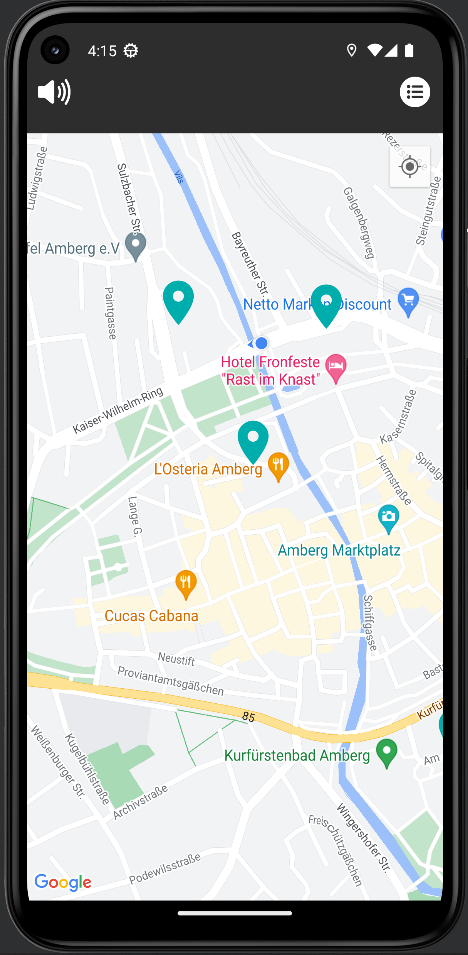
\includegraphics[width=0.3\linewidth]{app.png}
	\caption[Die Startseite der fertigen Anwendung, auf welcher man nun die Parkmöglichkeiten sieht und durch Klick auf einen Marker nähere Informationen findet. Oben rechts kann auch eine Liste der Parkmöglichkeiten aufgerufen werden. In der linken oberen Ecke kann der Ton an- und ausgeschaltet werden.]
	{Die Startseite der fertigen Anwendung, auf welcher man nun die Parkmöglichkeiten sieht und durch Klick auf einen Marker nähere Informationen findet. Oben rechts kann auch eine Liste der Parkmöglichkeiten aufgerufen werden. In der linken oberen Ecke kann der Ton an- und ausgeschaltet werden. (Quelle: Screenshot der erstellten Anwendung.)}
	\label{fig:app}
\end{figure}
\newpage
\section{Komponenten}
Die Komponenten bilden alle Funktionen der App, welche visuell auf der Benutzeroberfläche wahrgenommen werden. Neben der Anzeige der Elemente beinhalten sie aber dennoch auch Funktionalität, wie beispielsweise das Aufrufen von Methoden der Datenbank-Klasse ,DbConnectionService'. Alle Komponenten, mit Ausnahme der ,App', besitzen ein eigenes Interface. Dieses Interface beinhaltet alle Elemente, die als Properties in die Komponente hineingegeben werden und die jeweils dazugehörigen Typen. Properties können als Parameter an eine Komponente verstanden werden. Dies können neben Strings, Zahlenwerten oder boolschen Werten auch Funktionen oder andere Objekte sein.
\subsection{Komponente ,App'}
Die ,App'-Komponente kann sozusagen mit der ,main()'-Funktion anderer Programmiersprachen verglichen werden. Alles, was in dieser Funktion seinen Platz findet, findet sich auch in der Anwendung selbst wieder. Alle notwendigen Komponenten, die die Anwendung benötigt, werden hier eingefügt. 

Zu Beginn werden hier die Tabellen der Datenbank erstellt, sofern diese noch nicht existieren. Diese Komponente verwaltet die Daten. Die Informationen zu den Parkmöglichkeiten, die über die API abgerufen werden, werden zudem auch hier verwaltet. Durch den Hook ,useEffect' wird sichergestellt, dass die Daten nach einer bestimmten Zeit erneut abgefragt werden. Der Code hierfür kommt aus dem Internet und ist in \autoref{lst:useEffectApiData} zu sehen.

\begin{lstlisting}[caption={In diesem Hook werden nach der Zeit, welche sich hinter der Variable ,MINUTES\_MS' verbirgt, die Daten der API abgerufen, was über die Funktion in Zeile 3 geschieht. (Quelle: \cite{useIntervalCode})},captionpos=b, language=Java, label=lst:useEffectApiData]
	useEffect(() => {
		const intervalCall = setInterval(() => {
			dbConnectionService.getData();
		}, MINUTES_MS);
		return () => {
			clearInterval(intervalCall);
		};
	}, []);
\end{lstlisting}

Desweiteren gehehn auch die Daten des Eventhooks ,useGeofenceEvent', welcher in \autoref{geofenceEvent} erklärt wird, hier ein. Durch die Properties der anderen Komponenten werden die Daten dann an die richtigen Stellen gebracht. Wird ein Geofence betreten, so geschieht auch hier die Sprachausgabe. Der Button für das Ein- und Ausschalten des Tons befindet sich ebenfalls in der ,App'. Auch die Verwaltung des Tons liegt hier. Wird eine andere Ansicht geöffnet oder der Button zum Stummschalten der Sprachausgabe betätigt, so wird ein ,useEffect'-Hook getriggert, welcher die Sprachausgabe direkt beendet.

Neben verschiedenen ,set'- und ,get'-Funktionen, die für die Weitergabe von Daten zwischen Komponenten verantwortlich sind, befindet sich hier auch das Element, welches benötigt wird, um Toasts auszugeben. Alle Bestandteile in der ,<View>'-Komponente werden von ,<RootSiblingParent>' umrahmt, damit nachher an verschiedenen Stellen der Befehl aus \autoref{lst:toast} aufgerufen werden kann und somit in der Anwendung einen Toast anzeigt \cite{toastLibrary}.

\begin{lstlisting}[caption={Ein Beispiel des Aufrufs eines Toasts aus der Datei DbConnectionService. (Quelle: Eigene Implementierung)},captionpos=b, language=Java, label=lst:toast]
	Toast.show(errorMessages.noApiConnectionMessage, {
		duration: Toast.durations.LONG,
		position: Toast.positions.BOTTOM,
	});
\end{lstlisting}

\subsection{Komponente ,ParkingMap'}
Die wohl wichtigste Komponente der Anwendung ist die, welche die Karte beinhaltet. Diese findet sich hier. Zunächst wird beschrieben, welche Properties mitgeliedert werden. Hierzu ist es hilfreich, das zugehörige Interface ,IParkingMap' mit den Typen der Properties zu betrachten:
\begin{description}
	\item \textbf{handleParkingAreaId(id: number): void} \\ Hineingegeben wird eine Funktion ,handleParkingAreaId', welche nichts zurückgibt. Parameter ist hier ,id', was den Typ Nummer hat. Diese Funktion bringt die jeweilige ID der Parkmöglichkeit nach draußen in die ,App' und kann dort weiterverarbeitet werden.
	\item \textbf{handleParkingAreaDescription(parkingAreaDescription: boolean): void} \\ ,handleParkingAreaDescription' ist eine Funktion, welche nichts zurückgibt. Der Parameter dieser Funktion ist ein boolscher Wert namens ,parkingAreaDescription'. Diese Property hat in etwa denselben Nutzen, wie die eben beschriebene. Nur wird hier der ,App' mitgeteilt, ob die Beschreibung einer Parkmöglichkeit geöffnet werden soll oder nicht.
	\item \textbf{mapStyle: StyleProp<ViewStyle>} \\ Diese Property ist für das Design der ,ParkingMap' verantwortlich. Je nachdem, ob die Beschreibung der Parkmöglichkeit angezeigt wird oder nicht, ist die ,ParkingMap' größer oder kleiner.
\end{description}

Diese Komponete übernimmt die Anzeige der aktuellen Position des Nutzers und das Bilden der Geofences. Damit das funktioniert, benötigt man die Bibliothek Location von expo \cite{expoLocation}. Zur Nutzung von Geofences und der Anzeige der aktuellen Position wird die Erlaubnis des Nutzers für das GPS benötigt. Ohne diese Zustimmung wird dem Nutzer eine Meldung angezeigt, dass weder das Geofencing, noch die Anzeige der aktuellen Position funktionieren.

Um nun auch die Karte und die Marker an den Positionen der Parkhäuser anzeigen zu lassen, werden zusätzlich die Komponenten ,MapView' und ,Marker' der Bibliothek ,react-native-maps' benötigt. Je nach Gerät wird dann bei Android Google Maps und bei IOS Apple Maps verwendet. Um nun die Marker an den richtigen Stellen zu plazieren, wird die Liste aller Objekte der Parkmöglichkeiten mit der Funktion ,map()' durchgegangen und an jeder Stelle der Parkhäuser ein Marker gesetzt. Die Daten der Parkhäuser sind hier nicht aus der Datenbank, sondern aus dem Objekt-Array ,AllParkingAreas', welches in \autoref{AllParkingAreas} näher erklärt wird. Wird auf einen Marker geklickt, kommen die beiden Funktionen der Properties ins Spiel. Der Aufruf der Funktion ,handleParkingAreaId' mit der ID der angeklickten Parkmöglichkeit als Parameter lässt die ,App' wissen, welche Parkmöglichkeit angeklickt wurde. Wenn die Funktion ,handleParkingAreaDescription' mit dem Parameter ,true' aufgerufen wird, wird sichergestellt, dass sich dann immer die Beschreibung, welche in \autoref{fig:parkingAreaDescription} zu sehen ist, öffnet.

\begin{figure}[h!]
	\centering
	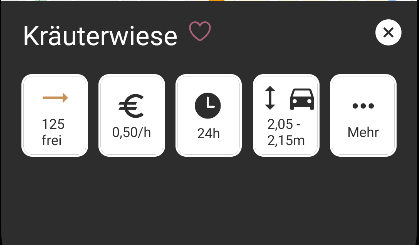
\includegraphics[width=0.45\linewidth]{parkingAreaDescription_component.png}
	\caption[Die Komponente ,ParkingAreaDescription', welche bei Klick auf einen Marker aufgerufen wird.]
	{Die Komponente ,ParkingAreaDescription', welche bei Klick auf einen Marker aufgerufen wird. (Quelle: Screenshot der erstellten Anwendung.)}
	\label{fig:parkingAreaDescription}
\end{figure}

\subsection{Komponente ,ParkingAreaDescription'}
\label{handleFunctions}
In dieser Komponente werden die relevantesten Daten einer Parkmöglichkeit in Kacheln angezeigt, wie in \autoref{fig:parkingAreaDescription} zu sehen ist. Auch für die Properties dieser Komponente gibt es ein Interface ,IParkingAreaDescription':
\begin{description}
	\item \textbf{dbConnectionService: DbConnectionService} \\ Dies ist eine Instanz des ,DbConnectionService', welche in der ,App' am Anfang erstellt wird. Diese Property ist für die Datenbankverbindung zuständig.
	\item \textbf{id: number} \\ Mit der Nummer ID kommt die ID der angeklickten Parkmöglichkeit in die Beschreibung. Nun kann mit Hilfe von ,dbConnectionService' in der Datenbank nach den passenden Daten gesucht werden.
	\item \textbf{geofenceEventData: IEventData[]} \\ Die Daten des Events ,useGeofenceEvent' werden in einem Objekt mit dem Interface IEventData gespeichert. Ein Array aus diesen Objekten bekommt auch die ,ParkingAreaDescription', damit unterhalb der Informationskacheln ein Button für die Navigation angezeigt werden kann, falls der Nutzer sich im Geofence einer Parkmöglichkeit befindet. Dieser Button ist auch auf \autoref{fig:parkingAreaDescriptionLetsGoButton} zu sehen.
	\begin{figure}[h!]
		\centering
		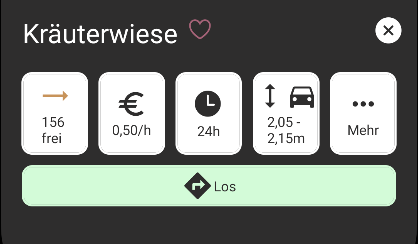
\includegraphics[width=0.45\linewidth]{parkingAreaDescriptionLetsGo_component.png}
		\caption[Die Komponente ,ParkingAreaDescription', welche bei Klick auf einen Marker aufgerufen wird.]
		{Die Komponente ,ParkingAreaDescription', welche bei Klick auf einen Marker aufgerufen wird. (Quelle: Screenshot der erstellten Anwendung.)}
		\label{fig:parkingAreaDescriptionLetsGoButton}
	\end{figure}
	\item \textbf{handleShowParkingAreaDescription(parkingAreaDescription: boolean): void} \\ Diese Funktion vom Typ ,void' mit der dazugehörigen boolschen Variable lässt die Beschreibung schließen. Wird dieser Wert auf ,false' gesetzt, so ist diese Funktion dafür zuständig, dies der App mitzuteilen, welche wiederum für die Anzeige dieser Beschreibung zuständig ist. Es wird geprüft, ob ,parkingAreaDescription' ,true' oder ,false' anzeigt. Bei ,true' öffnet sich diese Komponente, bei ,false' wird sie geschlossen. Dies geschieht beispielsweise, wenn der kleine weiße Kreis in der rechten Ecke in \autoref{fig:parkingAreaDescriptionLetsGoButton} betätigt wird.
	\item \textbf{handleParkingAreaDetails(parkingAreaDetails: boolean): void} \\ Der boolsche Parameter der Funktion zeigt an, ob auf den ,Mehr'-Button gedrückt wird. Ist der Button gedrückt worden, so wird die Komponente ,ParkingAreaDetails' geöffnet.
	\item \textbf{handleParkingAreaData(parkingAreaData: IParkingArea): void} \\ Diese Funktion beinhaltet ein Objekt des Typs ,IParkingArea', was das Interface für einen Eintrag einer Parkmöglichkeit ist und weiter unten beschrieben wird. Die Daten zur angeklickten Parkmöglichkeit gelangen so zur App.
	\item \textbf{handleParkingAreaDetailData(parkingAreaDetails: IParkingAreaDetails): void} \\ Diese Property macht genau das gleiche, wie die vorherige: Es werden Daten zu App getragen. In dem Fall handelt es sich um die Daten, wie voll die Parkmöglichkeit zum aktuellen Zeitpunkt ist.
	\item \textbf{handleDataBaseError(databaseError: boolean): void} \\ Diese Funktion beinhaltet einen boolschen Parameter, welcher der App mitteilt, wenn es zu einem Fehler in der Datenbank gekommen ist.
	\item \textbf{handleVolume(volume: boolean): void} \\ Öffnet man die Navigation mit dem ,Los'-Button oder die Details mit dem ,Mehr'-Button, so wird der App mitgeteilt, dass der Ton der Sprachausgabe beendet werden soll. Wird dies weggelassen, so wird die Sprachausgabe fortgesetzt, wenn man möglicherweise schon gar nicht mehr in der App, sondern schon bei der Navigation ist.
\end{description}

In der ,ParkingAreaDescription'-Komponente werden die Daten der angeklickten Parkmöglichkeit aus beiden Datenbanken abgerufen und dann in Kacheln dargestellt. Um den Code übersichtlicher zu gestalten, sind die Kacheln eine weitere Komponente: ,ParkingAreaDescriptionItemContainer', welche in \autoref{parkingAreaDescriptionItemContainer} näher beschrieben wird. Zudem kann hier das Parkhaus favorisiert werden, was direkt in die Datenbank eingetragen wird. Kommt es zu einem Datenbankfehler, so wird dies dem Nutzer über ein Altert mitgeteilt. Damit die Abfrage der Datenbank klappt und die Daten vor dem Rendern in den einzelnen Komponenten der ,ParkingAreaDescription'-Komponente stehen, muss die Abfrage asynchron ablaufen. Das heißt, dass gewartet werden muss, bis die Daten da sind, bevor sie angezeigt werden.

\subsubsection{Komponente ,ParkingAreaDescriptionItemContainer'}
\label{parkingAreaDescriptionItemContainer}
Diese Komponente ist die Kachel der ,ParkingAreaDescription'. Auch sie hat ein Interface für die Properties. Dieses beinhaltet aber nur den Text, einen oder zwei Namen für Icons und die Farbe der Icons. Ansonsten besitzt diese Komponente keinerlei Funktionalität. Sie ist nur für das Anzeigen zuständig und, dass in der ,ParkingAreaDescription'-Komponente weniger redundanter Code ist.

\subsection{Komponente ,ParkingAreaList'}
\label{parkingAreaList}
In \autoref{fig:ParkingAreaList} ist diese Komponente zu sehen. Hier sind die Parkmöglichkeiten mit Favoriten zuerst als anklickbare Kacheln alphabetisch aufgelistet. 
\begin{figure}[h!]
	\centering
	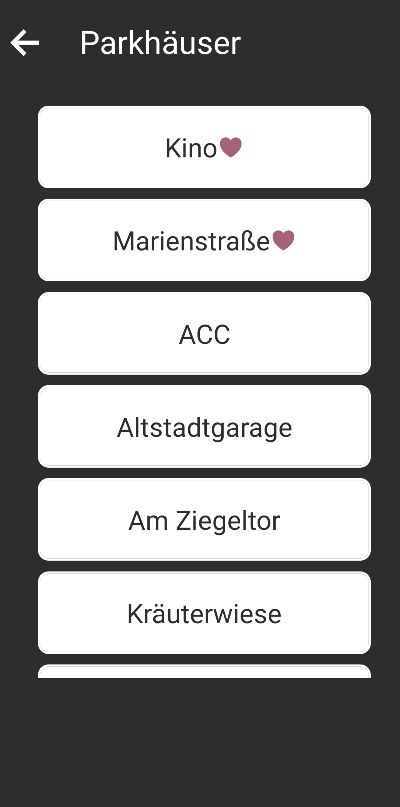
\includegraphics[width=0.33\linewidth]{parkingAreaList_component.png}
	\caption[Die Komponente ,ParkingAreaList', zu welcher man über einen Klick auf das Icon oben rechts in der App kommt. Die Liste ist mit Favoriten zuerst alphabetisch geordnet.]
	{Die Komponente ,ParkingAreaList', zu welcher man über einen Klick auf das Icon oben rechts in der App kommt. Die Liste ist mit Favoriten zuerst alphabetisch geordnet. (Quelle: Screenshot der erstellten Anwendung.)}
	\label{fig:ParkingAreaList}
\end{figure}

Die ,ParkingAreaList'-Komponente besitzt auch ein Interface für ihre Properties. So können die Typen dieser sichergestellt werden. Das Interface sieht folgendermaßen aus:
\begin{description}
	\item \textbf{dbConnectionService: DbConnectionService} \\ Diese Property vom Typ DbConnectionService ist wichtig für die Abfrage der Daten aus der Datenbank.
	\item \textbf{handleShowParkingAreaList(showParkingAreaList: boolean): void} \\ Diese Funktion ist dafür zuständig, die ,ParkingAreaList'-Komponente zu schließen, wenn man auf den Zurück-Pfeil drückt. In \autoref{fig:ParkingAreaList} ist die Liste mit dem Zurück-Pfeil zu sehen.
	\item \textbf{handleParkingAreaDescription(parkingAreaDescription: boolean): void} \\ Um nicht die Beschreibung ohne Daten zu haben, wenn die ,ParkingAreaDescription'-Komponente geöffnet ist, wenn man in die ,ParkingAreaList'-Komponente geht und wieder zurückkommt, wird die Beschreibung geschlossen, sobald der Zurück-Pfeil gedrückt wird.
	\item \textbf{handleParkingAreaDetails(parkingAreaDetails: boolean): void} \\ Diese Funktion erfüllt denselben Zweck wie ,handleParkingAreaDetails' in \autoref{handleFunctions}.
	\item \textbf{handleParkingAreaData(parkingAreaData: IParkingArea): void} \\ Auch hier tut die Funktion das Gleiche, wie ,handleParkingAreaData' in \autoref{handleFunctions}.
	\item \textbf{handleParkingAreaDetailData(parkingAreaDetails: IParkingAreaDetails): void} \\ In \autoref{handleFunctions} unter ,handleParkingAreaDetailData' ist beschrieben, was auch diese Funktion macht.
	\item \textbf{handleDataBaseError(databaseError: boolean): void} \\ Die Beschreibung dieser Property befindet sich in \autoref{handleFunctions} unter ,handleDataBaseError'.
\end{description} 

Die Überschrift dieser Komponente geht aus der Komponente ,ParkingAreaListHeadig' hervor, welche in \autoref{parkingAreaListHeading} zu finden ist. Ist bei der Datenbank-Abfrage in dieser Komponente kein Fehler aufgetreten, so werden die Namen der Parkmöglichkeiten als Flatlist dargestellt. Die Kacheln, in welchen sich die Namen der Parkmöglichkeiten befinden, gehen aus der Komponente ,ParkingAreaListItem' hervor. Klickt man auf eine dieser Kacheln, so kommt es zu einer weiteren Abfrage der Datenbank, wobei ,handleParkingAreaData' und ,handleParkingAreaDetailsData' der eben beschriebenen Properties mit den Daten gefüllt werden. Die Property ,handleParkingAreaDetails' wird dann auf ,true' gesetzt, um die Komponente in \autoref{parkingAreaDetails} zu öffnen. Je nachdem, ob ein Fehler bei der Datenbankabfrage auftritt, wird der Parameter in ,handleDataBaseError' auf ,true' oder ,false' gesetzt.

\subsubsection{Komponente ,ParkingAreaListItem'}
\label{parkingAreaListItem}
Diese Komponente besitzt, wie alle anderen auch ein Interface. Da es sich um anklickbare Kacheln handelt, muss man dieser Komponente die Funktion mitteilen, welche beim Klick ausgeführt werden soll. Für die Ausführung der Funktion braucht es zudem noch die ID der Parkmöglichkeit. Um den Namen und, falls die Parkmöglichkeit favorisiert wurde, ein Herz anzuzeigen, müssen auch noch der anzuzeigende Name als String und ein numerischer Wert für die Favorisierung mitgegeben werden. 0 heißt, dass die Parkmöglichkeit nicht unter die Favoriten fällt. 1 bedeutet, dass diese favorisiert wurde.

\subsection{Komponente ,ParkingAreaDetails'}
\label{parkingAreaDetails}
Wie bereits beschrieben, öffnet sich diese Komponente beim Klick auf ,mehr' in \autoref{fig:parkingAreaDescription} oder bei Auswahl einer Parkmöglichkeit in \autoref{fig:ParkingAreaList}. Diese Komponente dient lediglich zum Anzeigen von Daten. Dennoch kann auch hier eine Parkmöglichkeit zu den Favoriten hinzugefügt oder entfernt werden. Zu sehen ist diese Ansicht in \autoref{fig:parkingAreaDetails}.

\begin{figure}[h!]
	\centering
	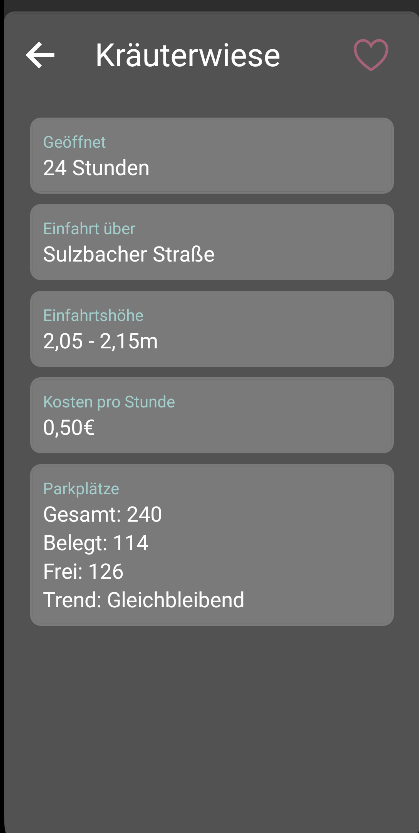
\includegraphics[width=0.33\linewidth]{parkingAreaDetails_component.png}
	\caption[Die Details zu einer Parkmöglichkeit. Hier werden alle vorhandenen Daten zur Parkmöglichkeit angezeigt. Sollte diese geschlossen sein oder aus anderen Gründen nicht befahrbar sein, wird dies dem Nutzer mit einem Text in einer roten Kachel mitgeteilt. Der Nutzer kann auch hier Parkmöglichkeiten favorisieren oder von den Favoriten entfernen.]
	{Die Details zu einer Parkmöglichkeit. Hier werden alle vorhandenen Daten zur Parkmöglichkeit angezeigt. Sollte diese geschlossen sein oder aus anderen Gründen nicht befahrbar sein, wird dies dem Nutzer mit einem Text in einer roten Kachel mitgeteilt. Der Nutzer kann auch hier Parkmöglichkeiten favorisieren oder von den Favoriten entfernen. (Quelle: Screenshot der erstellten Anwendung.)}
	\label{fig:parkingAreaDetails}
\end{figure}

Die Properties, welche durch das Interface ihren Typ erhalten, sind folgende: 
\begin{description}
	\item \textbf{dbConnectionService: DbConnectionService} \\ Diese Propertie ist dafür zuständig, dass beim Drücken auf das Herz in der oberen rechten Ecke eine Parkmöglichkeit in der Datenbank als Favorit oder kein Favorit eingetragen werden kann.
	\item \textbf{handleShowParkingAreaDetails(parkingAreaDetails: boolean): void} \\ Diese Funktion wird benötigt, wenn der Pfeil in der oberen linken Ecke gedrückt wird. Tut der Nutzer das, wo wird ,parkingAreaDetails' auf ,false' gesetzt und die Ansicht aus \autoref{fig:parkingAreaDetails} wird geschlossen.
	\item \textbf{parkingAreaData: IParkingArea} \\ Das Objekt, welches Parkhausdaten, wie die Einfahrtshöhe oder den Preis, beinhaltet.
	\item \textbf{parkingAreaDetailsData: IParkingAreaDetails} \\ Das Objekt, welches die Daten der API beinhaltet, welche unter ,Parkplätze' in \autoref{fig:parkingAreaDetails} dargestellt sind.
	\item \textbf{databaseError: boolean} \\ Ist diese Property ,true', so bekommt der Nutzer eine rot gefärbte Kachel mit einem Text angezeigt, der ihn darauf hinweist, dass die Daten nicht angezeigt werden können. In diesem Fall ist die Aktion zu wiederholen.
\end{description}

Da hier die Kacheln ebenfalls aus jeweils den gleichen ,View'-Komponenten und demselben Design bestehen, wurde hier wieder eine Komponente ,ParkingAreaDetailsItem' erstellt, welche sich darum kümmert, die Elemente schön anzuzeigen. Die Überschrift kommt ebenfalls durch die Komponente ,ParkingAreaListHeading' in \autoref{parkingAreaListHeading} zustande, wie die Überschrift in \autoref{parkingAreaList}.

\subsubsection{Komponente ,ParkingAreaDetailsItem'}
Diese Komponente ist ebenfalls nur zum Anzeigen von Dateien. Ihre Properties sind der Text, der in der Kachel jeweils oben kleiner angezeigt wird und jener Text, welcher etwas größer darin steht und anhängig von der angeklickten Parkmöglichkeit ist. Außerdem wird eine boolsche Variable hineingegeben, die dieser Komponente mitteilt, ob es sich um die Anzeige eines Fehlers handelt. Ist das der Fall, werden die Kacheln rot gefärbt.

\subsection{Komponente ,ParkingAreaListHeading'}
\label{parkingAreaListHeading}
Diese Komponente beinhaltet das Design der Überschrift, wie in \autoref{fig:ParkingAreaList} oder \autoref{fig:parkingAreaDetails} zu sehen. Als Property werden hier lediglich die Funktion, die beim Klick auf den Zurück-Pfeil erfolgen soll und der Text, welcher dargestellt werden soll, hineingegeben.

\section{Datenbankverbindung ,DbConnectionService'}
\section{Eventhook ,useGeofenceEvent'}
\label{geofenceEvent}
\section{Models}
\subsection{Interface ,IParkingArea'}
\subsection{Interface ,IParkingAreaDetails'}
\subsection{Interface ,IEventData'}
\section{Parkhausdaten ,AllParkingAreas'}
\label{AllParkingAreas}
\section{Weitere Hilfsmittel}
\subsection{Zentrale Verwaltung der Farben}
\subsection{Zentrale Verwaltung der Strings}